\documentclass{ximera}

\newcommand{\RR}{\mathbb R}
\renewcommand{\d}{\,d}
\newcommand{\dd}[2][]{\frac{d #1}{d #2}}
\renewcommand{\l}{\ell}
\newcommand{\ddx}{\frac{d}{dx}}
\newcommand{\dfn}{\textbf}
\newcommand{\eval}[1]{\bigg[ #1 \bigg]}


\outcome{Understand that we are approximating curves with straight lines.}
\outcome{Understand the connection between the Pythagorean Theorem and the length of curves.}
\outcome{Find lengths of curves both in terms of $x$ and $y$.}
  


\title[Dig-In:]{Length of curves}

\begin{document}
\begin{abstract}
We can integrate to find the length of curves.
\end{abstract}
\maketitle

Another geometric application of the integral is to find the length of
a curve.  We already know how to compute one simple arc length, that
of a line segment. If the endpoints are $(x_0,y_0)$ and $(x_1,y_1)$
then the length of the segment is the distance between the points,
$\sqrt{(x_1-x_0)^2+(y_1-y_0)^2}$.


\begin{image}
\begin{tikzpicture}
  \begin{axis}[
      xmin=0, xmax=7, ymin=0, ymax=5,
      clip=false,
      ticks=none,
      axis lines =center, xlabel=$x$, ylabel=$y$,
      every axis y label/.style={at=(current axis.above origin),anchor=south},
      every axis x label/.style={at=(current axis.right of origin),anchor=west},
      axis on top,
    ] 
    \addplot [very thick, penColor] plot coordinates {(3,2) (6,4)};
    \addplot [dashed, textColor] plot coordinates {(3,2) (6,2)};
    \addplot [dashed, textColor] plot coordinates {(6,4) (6,2)};
    \addplot[color=penColor,fill=penColor,only marks,mark=*] coordinates{(3,2)};  %% closed hole
    \addplot[color=penColor,fill=penColor,only marks,mark=*] coordinates{(6,4)};  %% closed hole
    \node at (axis cs:3,2) [anchor=east] {$(x_0,y_0)$};
    \node at (axis cs:6,4) [anchor=west] {$(x_1,y_1)$};
    \node at (axis cs:4.5,3.2) [penColor,anchor=east] {$\sqrt{(x_1-x_0)^2+(y_1-y_0)^2}$};
  \end{axis}
\end{tikzpicture}
\end{image}

If a function $f$ is differentiable, we can think of its graph as
being composed of infinitely many infinitesimal (directed) line segments with run
$\d x$, rise $\d y$, and length $\d s$.
\begin{image}
\begin{tikzpicture}
  \begin{axis}[
      xmin=2, xmax=3,ymin=1, ymax = 4,domain=2:3, axis lines =center,
      xlabel=$x$, ylabel=$y$,
      width=4in,
      height=2in,
      ticks=none, every axis y label/.style={at=(current
        axis.above origin),anchor=south}, every axis x
      label/.style={at=(current axis.right of origin),anchor=west},
      axis on top, ]
    \addplot [very thick, penColor,smooth]{16-19*x+8*x^2-x^3};
    \addplot [ultra thick, penColor2,->] plot coordinates {(2.4,2.656) (2.8,3.586)};
    \addplot [->, dashed,] plot coordinates {(2.8,2.656) (2.8,3.586)};
    \addplot [->, dashed,] plot coordinates {(2.4,2.656) (2.8,2.656)};
    \node at (axis cs:2.65,2.3) {$\d x$};
    \node at (axis cs:2.85,3.121) {$\d y$};
    \node at (axis cs:2.6,3.45) {$\d s$};
  \end{axis}
\end{tikzpicture}
\end{image}
By the \index{Pythagorean Theorem} Pythagorean Theorem, we have
\begin{align*}
	\left( \d s \right)^2 &= \left( \d x \right)^2 + \left( \d y \right)^2\\
	\left( \d s \right)^2 &= \left( 1 + \left( \frac{\d y}{\d x} \right)^2 \right) \left( \d x\right)^2\\
	\left( \d s \right)^2 &= \left( 1 + \left( f'(x) \right)^2 \right) \left( \d x\right)^2\\
	 \d s &= \sqrt{1 + \left( f'(x) \right)^2}\d x
\end{align*}
So, to find the length of a curve, we should accumulate these
infinitesimal lengths. This means that the length of the curve on the
interval $[a,b]$ is given by
\begin{image}
  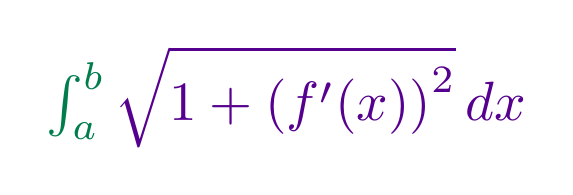
\begin{tikzpicture}[scale=2,every node/.style={transform shape}]
    \node at (0,0) {
      $\color{green!70!black!70!blue}\int_a^b \color{purple!50!blue!90!black}\sqrt{1 + \left( f'(x) \right)^2} \d x$
    };
  \end{tikzpicture}
\end{image}
which can be interpreted as
\begin{quote}
  \textbf{The length of a curve is given by the
    \textcolor{green!70!black!70!blue}{accumulated}
    \textcolor{purple!50!blue!90!black}{length determined by the
      instantaneous horizontal change and the instantaneous vertical
      change}.}
\end{quote}

\begin{warning}
  In order to be sure that our expression above actually computes the
  length, we need to also have the condition that $f'(x)$ is
  continuous on the (open) interval that we are integrating over.
\end{warning}

Let's see an example:
\begin{example}%% From guichard
  Find the length of $y = x^{\frac{3}{2}}$ from $x=0$ to $x=2$.
  \begin{explanation}
    Write with me:
    \begin{align*}
      \text{Length} &= \int_0^2 \sqrt{1+\left( \frac{\d y}{ \d x}\right)^2} \d x\\
      &= \int_0^2 \sqrt{1+\left(
        \answer[given]{\frac{3 x^{\frac{1}{2}}}{2}}\right)^2} \d x\\
      &= \int_0^2 \answer[given]{\sqrt{1+\frac{9x}{4}}} \d x
    \end{align*}
      Use the substitution $g = 1+\frac{9x}{4}$ to compute this integral:
      \begin{align*}
	\int_0^2 \sqrt{1+\frac{9x}{4}} \d x &= \frac{4}{9} \int_{\answer[given]{1}}^{\answer[given]{\frac{11}{2}}} g^\frac{1}{2} \d g\\
	&= \frac{4}{9} \left(\frac{2}{3}\right) \eval{g^{\frac{3}{2}}}_{\answer[given]{1}}^{\answer[given]{\frac{11}{2}}}\\
	&=\frac{8}{27} \left(\left(\frac{11}{2}\right)^\frac{3}{2} - 1\right)
      \end{align*}
  \end{explanation}
\end{example}

Most of the integrands arising in length calculations do not have
elementary antiderivatives, so oftentimes you will only be able to set
them up and estimate them numerically.

\begin{example}
  Estimate the length of the curve $y = \sin(x)$ from $x=0$ to $x =
  \pi$.  Truncate your answer at the hundredths place.
  \begin{explanation}
    Write with me:
    \begin{align*}
      \text{Length} &= \int_0^\pi \sqrt{1+\left( \frac{\d y}{ \d x}\right)^2} \d x\\
      &= \int_0^\pi \sqrt{1+\left(
        \answer[given]{\cos(x)}\right)^2} \d x
    \end{align*}
    This integral is hard for humans like us, but for our silicon
    friends, it is not so bad.  You can use a computer algebra system
    (or Wolfram Alpha) to approximate this to two decimal places:
    \[
    \text{Length} \approx \answer[given]{3.82}.
    \]
  \end{explanation}
\end{example}

Just like it was sometimes advantageous to integrate with respect to
$y$ in our area and volume calculations, it can also help us sometimes
in arclength calculations.  If you look back at how we calculated $\d
s$, you will see that we basically used the Pythagorean Theorem, and
pulled out a $\d x$.  So if $y = f(x)$, then $x = f^{-1}(y)$ and so
using the same reasoning as before
\[
\d s = \sqrt{1+\frac{\d x}{\d y}} \d y  = \sqrt{1+\dd[f^{-1}(y)]{y}} \d y
\]
\begin{image}
  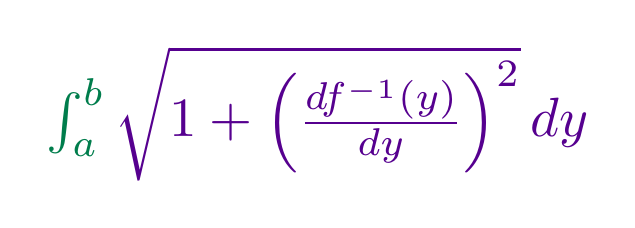
\begin{tikzpicture}[scale=2,every node/.style={transform shape}]
    \node at (0,0) {
      $\color{green!70!black!70!blue}\int_a^b \color{purple!50!blue!90!black}\sqrt{1 + \left( \dd[f^{-1}(y)]{y} \right)^2} \d y$
    };
  \end{tikzpicture}
\end{image}
which \textbf{still} can be interpreted as
\begin{quote}
  \textbf{The length of a curve is given by the
    \textcolor{green!70!black!70!blue}{accumulated}
    \textcolor{purple!50!blue!90!black}{length determined by the
      instantaneous horizontal change and the instantaneous vertical
      change}.}
\end{quote}

\begin{warning}
  In order to be sure that our expression above actually computes the
  length, we need to also have the condition that $\dd[f^{-1}(y)]{y}$ is
  continuous on the (open) interval that we are integrating over.
\end{warning}

\begin{example}
  Find the length of $y = \arcsec(e^x)$ from $x= 0$ to
  $x=\ln(\sqrt{2})$.
  \begin{explanation}
    This problem will be much easier if we work with respect to $y$. Write with me
    \begin{align*}
      y &= \arcsec(e^x)\\
      \sec(y) &= e^x\\
      \ln(\sec(y)) &= x.
    \end{align*}
    The limits of integration are
    \begin{align*}
      \arcsec(e^0) &= \answer[given]{0}\\
      \arcsec(e^{\ln(\sqrt{2})}) &= \answer[given]{\frac{\pi}{4}}
    \end{align*}
    So now write with me:
    \begin{align*}
      \text{Length} &= \int_0^{\frac{\pi}{4}} \sqrt{1+\left( \answer[given]{\tan(y)} \right)^2} \d y\\
      &=\int_0^{\frac{\pi}{4}} \answer[given]{\sqrt{1+\tan^2(y)}}\d y\\
      &=\int_0^{\frac{\pi}{4}} \answer[given]{\sqrt{\sec^2(y)}}\d y\\
      &=\int_0^{\frac{\pi}{4}} \answer[given]{\sec(y)} \d y\\
      &=\eval{\ln(\sec(x)+\tan(x))}_0^\frac{\pi}{4}\\
      &=\ln(\answer[given]{1+\sqrt{2}}).
    \end{align*}
  \end{explanation}
\end{example}
\end{document}
